% TEMPLATE for Usenix papers, specifically to meet requirements of
%  USENIX '05
% originally a template for producing IEEE-format articles using LaTeX.
%   written by Matthew Ward, CS Department, Worcester Polytechnic Institute.
% adapted by David Beazley for his excellent SWIG paper in Proceedings,
%   Tcl 96
% turned into a smartass generic template by De Clarke, with thanks to
%   both the above pioneers
% use at your own risk.  Complaints to /dev/null.
% make it two column with no page numbering, default is 10 point

% Munged by Fred Douglis <douglis@research.att.com> 10/97 to separate
% the .sty file from the LaTeX source template, so that people can
% more easily include the .sty file into an existing document.  Also
% changed to more closely follow the style guidelines as represented
% by the Word sample file. 

% Note that since 2010, USENIX does not require endnotes. If you want
% foot of page notes, don't include the endnotes package in the 
% usepackage command, below.

% This version uses the latex2e styles, not the very ancient 2.09 stuff.
\documentclass[letterpaper,twocolumn,10pt]{article}

\usepackage{usenix,epsfig,endnotes}
\usepackage{hyperref}
\usepackage{color}
\usepackage[backend=bibtex]{biblatex}
\bibliography{bibliography}

% Don't use monospace URLs.
\urlstyle{sf}

\definecolor{dred}{rgb}{0.8,0,0}
\hypersetup{colorlinks=true,urlcolor=blue,linkcolor=blue,citecolor=blue}

\begin{document}

%don't want date printed
\date{}

%make title bold and 14 pt font (Latex default is non-bold, 16 pt)
\title{
	\Large \bf Cartography: Global Censorship Detection \\
	over the RIPE Atlas Network
}

\author{
	Redacted for anonymization
% {\rm First Name}\\
% First Institution
% \and
% {\rm Second Name}\\
% Second Institution
% \and
% {\rm Collin Anderson}\\
% Annenberg School, University of Pennsylvania
}

\maketitle

% Use the following at camera-ready time to suppress page numbers.
% Comment it out when you first submit the paper for review.
\thispagestyle{empty}

\subsection*{Abstract}

As governments, ISPs and other intermedaries assert greater control over the
Internet, academic researchers and civil society organizations continue to face
difficulties in developing countermeasures.  While multiple initiatives promise
specially-designed censorship detection, no current project offers widespread
deployment or open access to granular datasets.
%
In order to foster broad, rapid and consistent measurements of censorship
events, we build on top of the RIPE Atlas network.  We propose strategies for
monitoring the reachability of vital services through an algorithm that balance
timeliness, diversity and cost.  We then apply these premises toward events in
Turkey and Russia in order to test our assertions, in the process uncovering
evidence of cooperation between a well-known blogging platform and government
authorities for purposes of faciliating the censorship of hosted content.

\section{Introduction}
%train of thoughts: talking about the recent popularity of censorship in the world and countires in
%africa and middle easts(cite news article) Then talk about the exsisting methods and briefly critic each onem then
%talk about what were the charactestics we were interested to have in current tools, then talk about
%Ripe atlas as a suitable tool, then talk about their issue related to cost function then talk about
%our contributions.

% talking about the scope of the problem
Tools for discovering censorship are essential considering their importance for journalists and
activists in many countires. Currently, the existaning infruastructures lack representetive(measurment machines) in
regions that they matter the most or they are not easy to use. 

Talking about the importance of RIPE Atlas in the past months. Refer to papers that used RIPE to collect data(\cite{lutu2014understanding} and \cite{brownlee2014searching}).

% Point out what problems the world is facing and how RIPE Atlas can help.

% Quick description of Atlas.
RIPE Atlas~\cite{atlas} is an Internet measurement network which was started in 2010 by RIPE NCC.
All measurement probes which constitute the network are run by volunteers.  Once a user connected
her probe to the network, it can be used for measurements and the user is also able to run custom
measurements by spending some of the network's currency, Atlas credits.  These credits are awarded
automatically based on the uptime of contributed probes.

% What kind of measurements does Atlas allow?
As of today, Atlas allows four types of measurements; ping, traceroute, DNS resolution, and X.509
certificate fetching.  All four measurement types can further be parameterised for more fine-grained
control.

% What are our contributions?  Is there more?
This work has three main contributions.
\begin{itemize}
	\item We evaluate the aptitude of RIPE Atlas for censorship analysis.
	\item We propose an algorithm to balance
	timeliness, diversity, and cost to facilitate effective censorship analysis.\footnote{All our
	code will be publicly available but we redacted the URL for anonymisation.}
	\item We present censorship analysis results based on several months of measurements.
\end{itemize}


\section{Related Work}
\label{related_work}
\begin{table*}[ht!]
\centering
\begin{tabular}{l|cccc}
\textbf{Platform} & \textbf{Flexibility} & \textbf{Coverage} &
\textbf{Blocking resistance} & \textbf{Main use} \\
\hline 
PlanetLab~\cite{planetlab} & High & Low/Medium & Medium & Network measurements \\
Atlas~\cite{atlas} & Low & Medium/High & Medium & Network measurements \\
M-Lab~\cite{dovrolis2010measurement} & Low & High & Medium & Network measurements \\
Tor~\cite{Dingledine2004} & Medium & Medium & Low & Low-latency anonymity \\
OONI~\cite{Filasto2012} & High & Low & Medium & Censorship analysis \\
Herdict~\cite{Herdict} & Low & Low/Medium & Low & Censorship analysis \\
OpenNet~\cite{opennet} & Low & Medium & High & Censorship analysis \\
\hline 
\end{tabular} 
\caption{Comparison between several popular censorship analysis platforms.}
\label{tab:comparison}
\end{table*}

% Longitudinal studies.
It is not difficult to conduct one-off censorship studies because censors
typically do not have sufficient time to react and thwart the research.
Longitudinal studies, on the other hand, are more challenging as they have to
be designed in a tamper-proof and sustainable way.  In 2007, Crandall et al.
proposed ConceptDoppler~\cite{Crandall2007}.  The design enables longitudinal
censorship analysis by detecting which keywords are filtered by the Great
Firewall of China (GFW) over time.  More recently, CensMon was introduced by
Sfakianakis et al. in 2011~\cite{Sfakianakis2011}.  CensMon is a web censorship
monitor which is run on top of PlanetLab~\cite{planetlab}.  Most recently, in
2012, Filast\`{o} and Appelbaum presented OONI~\cite{Filasto2012}.  In
contrast to CensMon and ConceptDoppler, OONI is deployed and has been used
successfully.\footnote{Gathered reports are available online at:
\url{https://ooni.torproject.org/reports/}.}  In parallel to the open platforms
discussed above, proprietary platforms exist~\cite{hwang2007herdict,opennet}.


% Comparison to other projects.
Table~\ref{tab:comparison} contains a comparison between popular and deployed
platforms which are or can be used for censorship analysis.  Our comparison is
based on \emph{flexibility} (i.e., how many types of measurements can be run),
\emph{coverage} (i.e., how many probes in how many countries are available),
and \emph{blocking resistance} (i.e., how easy it is for censors to disable the
respective platform).  We qualitatively compare all platforms and assign them
the labels ``Low'', ``Medium'', or ``High''.  Note that we do not propose
Atlas as \emph{replacement} for any existing censorship measurement platforms.
Instead, we see it as a \emph{complement} that contributes to the already
existing and growing landscape of initiatives.

% Side channel measurements.
% TODO - Are there more papers we are missing?
Additionally, in the absence of deployed platforms or other means to access machines inside
censoring countries, censorship analysts have resorted to exploiting TCP/IP
side channels.  In particular, Ensafi et al. demonstrated that it is possible
to measure intentional packet dropping without controlling either the source or
the destination machine~\cite{Ensafi2014}.

% Previous Atlas censorship analysis.
Atlas has already been used as platform for censorship analysis outside an
academic setting.  In 2014, Maass used Atlas to find inconsistencies in the DNS
records and X.509 certificates for torproject.org~\cite{Maass2014}.  In the
same year, Bortzmeyer and Aben independently discussed Internet censorship in
Turkey~\cite{Bortzmeyer14,Aben14}.  While we discuss the same topic in
Section~\ref{sec:case_studies}, we do so with significantly more data and in a
more rigorous fashion based on the privilege of time.
\section{Framework Structure}
\label{sec:framework}
We now discuss Atlas' aptitude as censorship analysis platform and continue by
presenting \textsf{Cartography}, our censorship analysis framework which is
based on RIPE Atlas.

\subsection{RIPE Atlas Background}
% Some basic information about Atlas.
Having been founded in 2010 by RIPE NCC, Atlas~\cite{atlas} is a globally
distributed Internet measurement network consisting of probes run by
volunteers.  Once a user connected her probe to the network, it can be used for
measurements and the user is also able to run custom measurements by spending
some of the network's currency, Atlas credits.  These credits are awarded
automatically based on the uptime of contributed probes.  Measurements can be
run either over the web frontend, or over a HTTP-based API.

% Geographic and topological distribution.
An ideal censorship measurement platform features high geographic and
topological diversity, thereby facilitating measurements in any region where
censorship occurs.  While Atlas probes are distributed throughout the world,
there is a significant bias towards the U.S. and Europe as can be seen in
Figure~\ref{fig:probe_distribution}.  As for Atlas' topography, only 68
autonomous systems contain 40\% of all Atlas probes with the three most common
autonomous systems being 7922 (4.4\%, Comcast Cable Communications), 3320
(3.2\%, Deutsche Telekom), and 6830 (2.8\%, Liberty Global Operations).  While
not optimal, most censoring regions still contain at least several probes.

\begin{figure}[t]
\centering
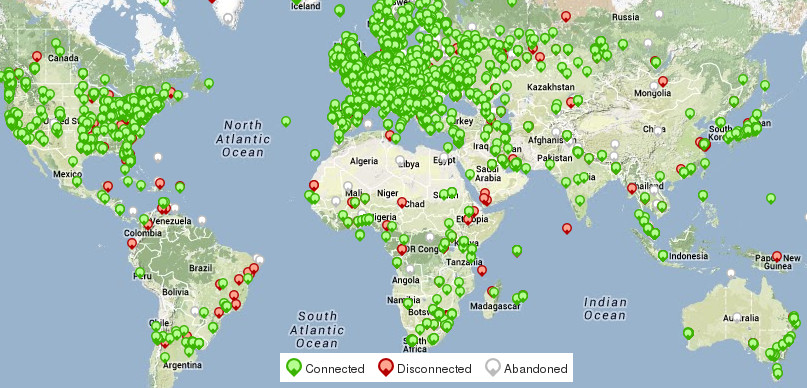
\includegraphics[width=0.48\textwidth]{diagrams/probe_distribution.jpg}
\caption{The geographic distribution of Atlas probes as of May 2014.  Green
icons represent active probes and red icons represent probes which are
currently offline.  The distribution is biased towards the U.S. and Europe.}
\label{fig:probe_distribution}
\end{figure}

% What kind of measurements does Atlas allow?
As of May 2014, Atlas allows four types of measurements; ping, traceroute, DNS
resolution, and X.509 certificate fetching.  All four measurement types can
further be parameterized for more fine-grained control.  HTTP requests are not
possible at this point due to concerns.  While Atlas clearly lacks the
flexibility of comparable platforms (see Table~\ref{tab:comparison}), it makes
up for it with comparably high diversity and its continued growth.  After all,
we do not expect Atlas to replace existing platforms such as OONI but rather to
\emph{complement} them.

% TODO - Should we talk about our crappy command-line interface?

% We also need to mention how you can stablish a big experiments using RIPE.
% And mention about the propblem of how you frist need to submit your
% experiments and then it will give you predicted cost. This way we can move to
% cost function.
As briefly mentioned above, Atlas' measurement have to be paid with so-called
credits.  The exact ``price'' of a measurement depends on the measurement type,
its parameters, and the destination(s).

\subsection{Ethical Aspects}
% The problem.
Atlas was not designed as censorship analysis platform and accordingly, its
volunteers likely do not expect that their probes will be used for such
purposes.  Careless measurements could attract a censor's attention and cause
repercussions for the respective probe operator.

% How we justify our research.
Recall that Atlas' measurement types are limited to ping, traceroute, DNS
requests and X.509 certificate fetching.  As of May 2014, it is not possible to
create HTTP requests or engage in actual, meaningful communication with
arbitrary destinations which limits the damage caused by reckless measurement.
Nevertheless, we acknowledge that care must always be taken and hope to initiate
further ethical discussions.


% \section{Factors in Assessing Measurement Validity}

\subsection{Precautions and Considerations}

Iran imposes a multi-layer content filtering apparatus through both direct control of network infrastructure, as well as regulatory mandates under telecommunications licensing regimes. At nearly every level of connectivity, traffic transiting across the boundaries of Iran's service providers and exchange points is subject to the possibility of monitoring or disruption. In most cases, primary form of disruption appears to be either inspection of HTTP headers or DPI-based DNS interception and poisoning  in the path of the international gateway administered by the Telecommunications Company of Iran (TCI). While these mechanisms are effective in enforcing the country's broad range of content restrictions, the apparatus has been demonstrated to be blind to requests that deviate slightly from expectations, including TCP-based DNS queries or web requests with improper spacing \cite{aryan2013internet}.

Despite their distribution across a diversity of countries and networks, RIPE Atlas may not fully reflect the Internet as it is experienced by the public, as probes neither fully emulate either the position nor the configuration of an average user. For example, while Iran has blocked access to YouTube continually since it was used to document post-election protests in June 2009, out of 22 probes queries, 10 probes covering 7 ASNs could successfully negotiate a SSL connection to the site. Moreover, Iran has a history of aggressively disrupting access to the Tor network through deep packet inspection, and has long filtered the project's site. However, while social media platforms and circumvention tools, like Balatarin and Ultrasurf, are subject to DNS interception, torproject.org from the perspective of Atlas is not. Based on TCP traceroutes to addresses with torproject.org DNS A record, restrictions on SSL connectivity are instead accomplished through IP blocking implemented within the TCI.

Incongruencies across probes and deviations from observations are an inevitable a product of the high rate of placement of Atlas probes on commercial and academic networks, as well as their use of a non-Windows operating system. These institutions may have alternative network connectivity that is faster and less highly regulated than consumer networks. Additionally, filtering mechanisms may rely catching plaintext requests or headers sent in the clear, such as TLS's SNI string, as their means to restrict access to SSL content. 

\subsection{Consensus Building}

The international distribution of web services, for purposes of performance, failover and load balancing, has created additional complexity in the determining whether answers received over the Internet are genuine. While SSL and DNSSEC utilize third-party trust to validate answers, Certificate Authorities have been previously compromised by state and non-state actors, and DNSSEC is not widely implemented. In order to validate answers within the Atlas network, we use a cross-country comparision of responses to queries. This methodology assumes that states that interfere with connectivity do not coordinate strategies internationally. States and Internet service providers institute different approaches to content-filtering for purposes of localization, infrastructure or even the monetization of blocked traffic. Furthermore, surveillance is more effective when the public is unaware of the practices and technologies employed against them, placing an strong incentive on secrecy and narrow targeting. Therefore, as a simple test of validity, we count the number of countries or ASNs that an answer, such as an A record or a certificate hash, is seen, and find the mean across all answers. Any response with fewer than the mean number of jurisdictions is treated a potentially aberrant and flagged for further investigation.


\section{Case Studies}
\label{sec:case_studies}

After having presented our measurement platform which is built on top of RIPE's
Atlas, we now evaluate it empirically by discussing two cases of large-scale
censorship we analyzed.  In particular, Turkey's ban of Twitter in
Section~\ref{sec:turkey} and Russia's ban of LiveJournal~\ref{sec:russia}.

% *** Can I try to negotiate with all dir authorities?

\subsection{Turkey's Ban of Twitter}
\label{sec:turkey}

Beginning March 20, 2014, social media users began to report limitations on the
availability of Twitter across the Turkey's Internet Service Providers.
YouTube and Twitter had both become the target of condemnation by Prime Minister
Erdogan.  Eventually, the Turkish government's Information
and Communication Technologies Authority (BTK) mandated the filtering of
Twitter on national ISP.

Turkey's Internet filtering has previously been connected to DNS tampering and
IP blocking \cite{akdeniz2010report}, which both fall under the measurements
possible through Atlas.  Upon news of the Twitter ban we started periodic
measurements over Atlas.  Through the ten probes covering nine ASNs, we
scheduled hourly measurements of local DNS answers, SSL connectivity, and
Traceroute reachability for Twitter, YouTube, Google Public DNS and the Tor
Project.  As illustrated in Figure~\ref{image:tr-social_media_filtering}, we
found at least six shifts in content restrictions and blocking strategies
within a two week period.

\begin{figure*}
  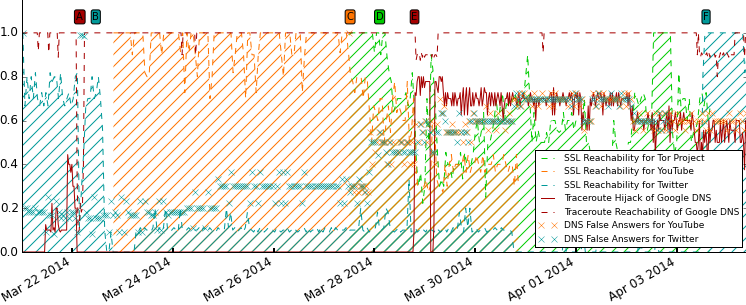
\includegraphics[width=\textwidth]{resources/tr-20140321-20140407-social_media_filtering.png}
  \label{image:tr-social_media_filtering}
  \caption{Disruption of Social Media Platforms in Turkey, March -- April 2014}
\end{figure*}


While the BTK and compliant ISPs rely on DNS manipulation and IP blocking, it
appears that the former is more popular.  As of April 24, 2014, the
Turkish-language anti-censorship site \textit{Engelliweb}, which tracks
addresses of blocked content, only lists 167 IP addresses restricted in
country, compared to 40,566 domain names \cite{engelliweb}.
% The popularity of content distribution networks
% and shared hosting easily makes address-based blocking either overbroad,
% creating collateral damage from restricting all domains and content on a shared
% host, or inefficiently narrow. Iranian authorities reportedly faced an aspect
% of this in October 2012, when an attempt to block  YouTube was blamed for
% week-long disruptions on access to Gmail, likely a result of shared
% infrastructure and addresses across Google's services \cite{bbc2012gmail}.
In absence of address blocking or HTTP filtering, users that received valid DNS
answers for Twitter's domain names could browse without further interference.
As a result, foreign DNS servers quickly became both a circumvention mechanism
and a political statement, with the addresses of alternative services offered
by Google and OpenDNS reportedly graffitied across the the country in protest
of the ban.

% The ease and rate that users were appeared to be bypassing the filters, by some
% indications more tweets were sent after the restrictions than before, prompted
% broader crackdown by authorities.
On the morning of March 22nd (see Figure~\ref{image:tr-social_media_filtering},
Event A), between 01:00 and 02:00, backbone providers Tellcom Iletisim
Hizmetleri and Turk Telekom began disrupting Google's Public DNS service
through the IP blocking of its two prominent addresses (8.8.8.8 and 8.8.4.4).

% This restriction would have disrupted access to filtered and non-filtered sites
% alike through interfering with the translation of names to Internet-routable
% addresses. Use of Google's DNS is commonplace in the country, and not
% necessarily indicative of an intent to circumvent filters. By some metrics
% 18.3\% of Internet users in Turkey rely on Google Public DNS
% \cite{ispcolumn2013googledns}. Given this cost, within hours,
By 6:00 the same morning, the DNS blocking had been removed across all ISPs.
Instead, to buttress the restrictions, providers shortly began to drop all
outgoing traffic to addresses associated with the twitter.com domain,
regardless of port, protocol or provider (\textbf{Event B}). By 16:00 of that
day, no Atlas probe could directly negotiate an SSL connection with Twitter
until the removal of the ban nearly two weeks later.

On March 27 (\textbf{Event C}), after recordings were posted of Turkish
national security officials discussing possible military action against Syria,
YouTube was blocked through false answers to DNS for the youtube.com domain.
Within the Atlas network, this restriction appears as slow decline in the
number of probes able to establish a connection to the media platform. However, unlike Twitter, a
significant minority of probes remained able to communicate with YouTube.
% Google's infrastructure presents substantial risk of collateral damage that
% could result from address or network prefix restrictions, which were not
% present with Twitter, and thus clients that were able to receive a valid
% address could reliably bypass the ban.

% Although the BTK is alleged to have ordered the installation of deep packet
% inspection equipment for purposes of lawful interception and censorship
% \cite{kirlidog2011deep}, restrictions on circumvention and anonymizations tools
% appear to have been limited to the filtering of services' websites.
Beginning
March 28th 19:00, Atlas probes in-country began fail to establish an SSL
connections to torproject.org (\textbf{Event D}). However, this restriction
neither included IP restrictions, nor was there evidence of interference with
the accessibility of the network. Atlas probes could continue to negotiate
valid connections to Tor's Directory Authories. Throughout the increased
manipulation of local DNS services, nearly half of the Atlas probes remained
connected due to their use of foreign DNS services.
% More aggressive
% restrictions were perhaps inevitable due to international attention on the
% rapid adoption of circumvention tools and Google Public DNS as an indicator of
% the futility of the ban.

\begin{figure*}
  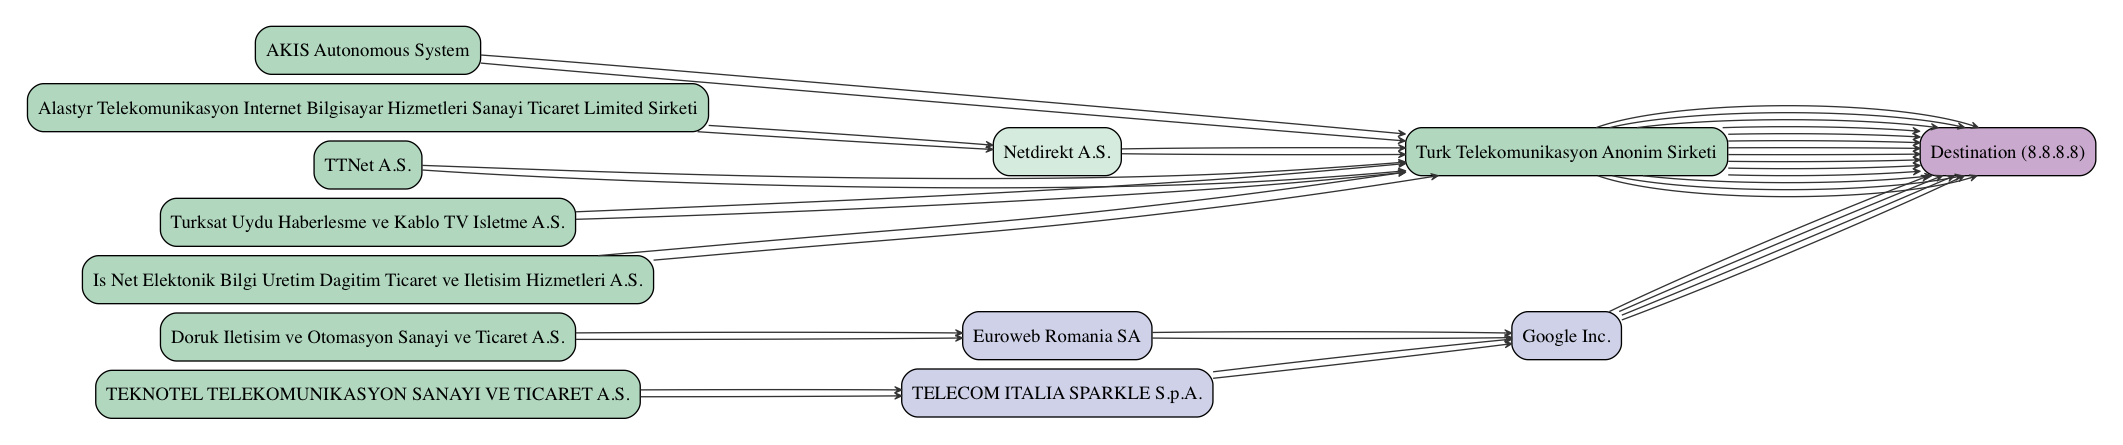
\includegraphics[width=\textwidth]{resources/traceroute-TR-google_public_dns-20140330-hijack.png}
  \label{image:tr-ttnet_hijack}
  \caption{Turkish Telecom (AS9121) Hijack of Google Public DNS Traffic, March 30 2014}
\end{figure*}

On the evening of March 28th, hosts querying foreign-based DNS servers began to
receive the same false answers as those provided domestically, leading to a
rapid drop in reported availability of YouTube and Tor (\textbf{Event E}). A
publicly-available traceroute measurement scheduled on the Atlas network by
third-parties against Google's Public DNS returned idiosyncratic and
spontaneous shifts in Turkey's network topology timed in relation to these
changes. These changes appeared within traceroutes as a shortening in the
number of hops to Google with a multifold reduction in traffic latency and the
absence of international hosts in path. The core telecommunications provider
Turk Telekom had begun to reroute traffic destined for Google to a local DNS
server, Figure~\ref{image:tr-ttnet_hijack}. Only TEKNOTEL Telekom maintained
consistently valid routes for Google Public DNS, through Telecom Italia
Sparkle, however, two days later Doruk \.{I}leti\c{s}im and Net Elektronik
Tasar{\i}m reestablished connectivity through Euroweb Romania. Turk Telekom's
redirection was finally removed late on April 7.

By April 3th, despite continued hijacking of Google's Public DNS for filtering
purposes and interference with YouTube, Twitter was unblocked for all probes
(\textbf{Event F}).

% % % % % % % % % % % % % % % % % % % % % % % % % % % % % % % % % % % % % % % %
\subsection{Private Sector Cooperation in Russian Censorship of Alexei Navalny}
\label{sec:russia}
% % % % % % % % % % % % % % % % % % % % % % % % % % % % % % % % % % % % % % % %

% Concurrent to broader restrictions on independent media, on March 13, 2014,
% Russia's Federal Service for Supervision in the Sphere of Telecom, Information
% Technologies and Mass Communications (Roskomnadzor) announced the blacklisting
% of opposition figure Alexei Navalny's LiveJournal blog, due to claimed
% violations of the terms of his house arrest. Shortly after the order was
% issued, Russian social media and state news agencies reported that access to
% the entirity of LiveJournal had been temporarily disrupted on some Interent
% providers due to their inability to distinguish traffic to different blogs
% within the site \cite{itar2014livejournal}. Overblocking has proven a recurrent
% issue in Russia. When a regional ISP, Netis Telekom, previously blocked the
% full site while complying with a court order against a neo-nazi blog,
% LiveJournal's Russian Director Ilya Dronov attributed the event to several
% ISPs' reliance on IP-based filtering and the inclusion of IP addresses within
% court orders \cite{leta2012livejoural}. 

On March 13, 2014, Russian authorities ordered the blacklisting of opposition
figure Alexei Navalny's LiveJournal blog.

% At the same time as Navalny's censorship, four opposition news portals were
% filtered based on the allegations that they called for ``illegal activity and
% participation in mass events that are conducted contrary to the established
% order,'' including grani.ru \cite{ibtimes2014russia}. As with Turkey, Russia's
% content restrictions have previously been attributed to DNS poisoning and IP
% filtering, presenting the same potential circumvention strategies and
% measurement opportunities \cite{rugovdns, verkamp2012inferring}. However, with
% a random sample of 255 probes across 147 ASNs in Russia, only 38 probes on 20
% ASNs received aberrant DNS answers. Within this subset, probes received a
% diverse, consistent selection of ten unique addresses, including two within
% RFC1918, private network address space (10.52.34.222 and 192.168.103.162). A
% greater selection, 40 probes across 23 ASNs, of traceroutes to the port 80 for
% the primary address associated with Grani as of April 30 (23.253.120.92) failed
% within Russia network space. Based on Russian filtering documentation efforts,
% the order that restricted Grani identifies at least fourteen addresses
% connected with the site \cite{antizapret2014}. An additional address that
% appears in the Grani order was found blocked on 36 probes and 22 ASNs,
% highlighting inconsistency in implementation and upkeep.
At the same time, four news portals were filtered which includes
grani.nu~\cite{ibtimes2014russia}.  Similar to Turkey, Internet filtering in
Russia is frequently conducted by IP blocking and DNS
poisoning~\cite{rugovdns,verkamp2012inferring}.  However, with a random sample
of 255 probes across 147 ASNs in Russia, only 38 probes on 20 ASNs received
aberrant DNS answers. Within this subset, probes received a diverse, consistent
selection of \emph{ten unique addresses}, including two within RFC1918, private
network address space (10.52.34.222 and 192.168.103.162). A greater selection,
40 probes across 23 ASNs, of traceroutes to the port 80 for the primary address
associated with Grani as of April 30 (23.253.120.92) failed within Russia
network space. Based on Russian filtering documentation efforts,

In contrast to Grani, a locally resolved DNS query for navalny.livejournal.com
over 255 probes on 146 ASNs received a consistent reply of 208.93.0.190, which
matched answers regionally with only one anomalous response, a formerly valid
address. The blocking of Navalny's blog must be different from Grani. While the
returned DNS A record of 208.93.0.190 falls within a network prefix owned by
LiveJournal Inc. (208.93.0.0/22), within the 1462 LiveJournal subdomains in
Alexa's Top 1 million list, 1450 blogs resolved another address, 208.93.0.150.
Both hosts appear to front servers for the LiveJournal platform, as they return
the same SSL Certificate and host the same content. Requests to 208.93.0.150
with a HTTP Host header set to navalny.livejournal.com retrieves the correct
content and non-blacklisted content is retrievable through 208.93.0.190.

As of April 2014, only five subdomains on livejournal.com could be found whose
DNS A records resolved to the address 208.93.0.190, Figure
\ref{lj-blocked-blogs}, four of which are listed within Alexa's top sites. All
the blogs found on this alternative host have been publicly declared by Russian
authorities as in violation the country's media laws for promotion of political
activities or extremism, and two are listed within publicly-available filter
site lists. 

\begin{figure*}
  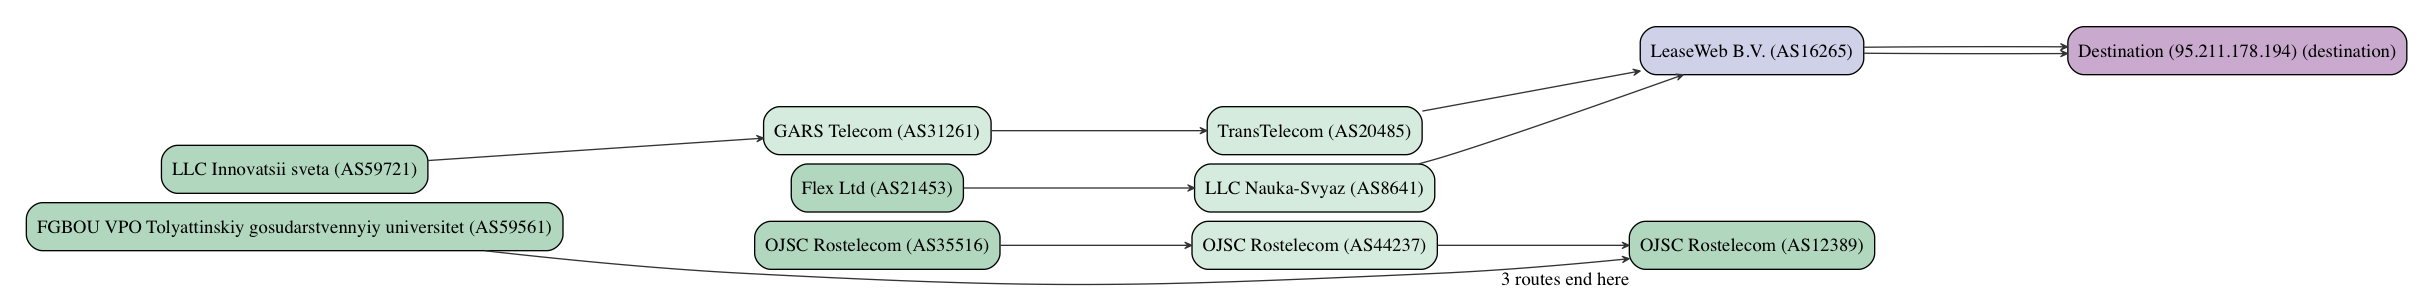
\includegraphics[width=\textwidth]{resources/atlas_cache-results-measurement_id-1663748.png}
  \label{image:ru-grani-hijack}
  \caption{Rostelecom (AS12389) Hijack of grani.ru Traffic, April 30 2014}
\end{figure*}

Based on timing, publicly-available history, available domain names records,
and Atlas network measurements, it appears that a host was specially
established to faciliate Russian censorship of the LiveJournal platform.
%potentially based on interest by the service to mitigate further overblocking
of the platform. Using HTTPS Ecosystem Scans as a metric of accessibility
\cite{projectsonar}, the LiveJournal frontend at 208.93.0.190 came online
between February 10 and February 17, with the address otherwise unused until
then. Two months later, the Ukrainian LiveJournal blog `Pauluskp'
(pauluskp.livejournal.com), which had covered Russian involvement in Crimea,
was filtered with the administrative order listing an IP Address of
208.93.0.190. However, as recently as six days before, the blog was recorded as
pointing to the main LiveJournal host. Similarly, the movement of Navalny's
blog was noticed within social media \ref{miptru2014}. It appears that in the
lead up to or at the time of filtering orders, LiveJournal coordinates with
authorities to alter the DNS A record for blogs designated by Roskomnadzor, in
order to segregate blacklisted content from the rest of the platform [6].

\begin{table}
    \begin{tabular}{| l | c | c |}
        \hline
        Subdomain & Language & Roskomnadzor\\
        \hline
        drugoi-nnover & Russian & Yes\\
        m-athanasios & Russian & Yes\\
        imperialcommiss & Russian & Yes\\
        pauluskp & Russian & Yes \\
        navalny & Russian & Yes \\
        \hline
    \end{tabular}
    \label{table:lj-blocked-blogs}
    \caption{LiveJournal DNS A Records of 208.93.0.190}
\end{table}

Segregated LiveJournal content and a blacklisted addresses are subject to an
additional, unknown method of network-layer interception performed within the
backbone network of Rostelecom (AS12389). While LiveJournal blog content is not
accessible over HTTPS, frontend hosts offer SSL services for the purpose of
securing the transmission of user credentials. As of April 28, 255 of 343
probes within Russia were able to retrieve a valid and consistent LiveJournal
SSL Certificate from the alternative LiveJournal host by address. Another 78
probes returned either irregular responses or failed to connect, of which 40
probes on 29 ASNs returned SSL certificates with common name or locations
fields attributed to Russian ISPs. Based on HTTPS data, the four aberrant
certificates captured have been seen previously on seven Russian addresses
belonging to the State Institute of Information Technologies, Rostelecom and
Electron telecom network. Three of these hosts are responsive and still match
certificates, two are generic ISP homepages and one notifies of the blocking of
the site `rutracker.ru.' Other measurements that are unresponsive could be
indicative of port blocking by other intermediaries or the redirection of
traffic to a server that is not listening for SSL connections.

The invalid certificates indicate that an intermediary in transit has
intercepted or redirected the traffic out of its normal path to a third-party
server controlled by Russian entities. This approach is different from the
normal man-in-the-middle approach seen in countries such as Iran and Syria, and
ellucidates the potential for Russian ISPs to falsify content or gather user
credentials. This behavior is not limited to protocol or port, although the end
host appears to be only responsive to TCP requests, Figure
\ref{image:ru-grani-hijack}. Hollistic interference suggesting the redirection
at the network layer, rather than application-based decisions or termination of
traffic associated with deep packet inspection. Moreover, adjacent addresses
within the same network and others destinations, such as the normal frontend
for LiveJournal traverse a valid international path. Instead, blacklisted
	traffic appears to be coerced into a path controlled by Rostelecom that is
	otherwise not taking for destinations within the same network, indicating a
	narrowly-crafted interference with normal routing through false
	advertisements or forwarding.


%\section{Discussion}

\subsection{Ethical Considerations}

% TODO Roya will fill this up later.
The problem: we might endanger probe contributors by running censored queries over their probes.
Contributors probably don't expect that their probe is used for censorship analysis.

Our justification: Plausible deniability, we are limited to X.509/DNS/ping/traceroute.  We are not
claiming that everything is OK.  Instead, we encourage further discussion.

\subsection{Conclusion}

% The implementation of the March 22nd address blockage of Google Public DNS falsely appears based on timing metrics to be a route hijack. While retaining valid routes across the international frontier into Google's network, the round trip times for several probes dropped precipitiously preceeding their blockage. For one of the last probes blocked, the time taken to reach the last hop out of the country had declined from 60.893 ms to 23.164 ms. However, by March 28,

These findings contribute to broader discussions on anticensorship strategies.  Collateral damage and level of difficulty appears to have shaped the implementation of Turkey and Russia's filtering mandates and responses to circumvention. The quick removal of restrictions on Google Public DNS, and then later attempts to impersonate the service, demonstrated that enforcing an absolute prohibition on filtered content was not worth incurring the cost of disrupting access a large portion of the population. While alternative strategies were possible with Twitter, due to its addressing schema, historical lessons from other countries' attempt to filter YouTube has run into the complexity and interdependency of Google's services. Where there are high collateral costs, such as with YouTube in Turkey and LiveJournal in Russia, authorities have been forced to either limit their restrictions or find cooperative arrangements with the platform. 

Filtering apparatuses may be more effective at disrupting easy access to marginal content or coercing content providers into compliance, than actual denial of information for a sufficiently motivated user. Neither Turkey or Russia's filtering apparatuses appears to have been designed to handle widespread intent to circumvent, particularly when more aggressive restrictions could incur collateral damage. When foreign DNS requests are allowed and not subject to deep packet inspection, circumvention is simple. Upon initial DNS restrictions, only 20\% of probes in Turkey were no longer able to connect to Twitter. The remainder either utilized foreign DNS servers or tunneled traffic out of country by other means, thereby creating inconsistent reports of accessibility. This may reflect a common experience for a large portion of the Turkish population, given previous accounts of the adoption of foreign DNS servers. Direct access to  was only effectively cut off by March 23, when traffic to the platform blocked by IP address. Even with the BGP hijack and local DNS interference, YouTube remained accessible for 40\% of Atlas probes attributed to Turkish networks. 

Finally, due to Turkish and Russian telecommunications companies reliance on blocking network reachability and interfereing with name translation, rather than traffic inspection, the Atlas network was well positioned for both blocking incident. If authorities had utilized HTTP inspection, Atlas would not have been capable of documenting either event. However, without secondary investigation and additional restrictions, initially produced results would have called into question the veracity of accounts of Twitter's filtering. Other inconsistences remain unaccounted for. 

In Atlas's view, several networks within Turk Telekomunikasyon had already began to filter YouTube by the time measurements had been queued at March 21. These measurements precede public accounts and broader censorships by the several days. The differences of experiences of filtering rules is in part a product of Turkey's decentralized network infrastructure, differing Iran and Syria, which maintain monopolistic over international gateways. Content restrictions appear to be instituted by court or administrative order, which are complied with at differing rates. However, this also reflects a disparity between the network conditions of the probes and those of the average user. At the time of blocking, 70\% of probes relied on a DNS server outside of the country, and at least one had at various times tunneled all traffic by unknown means. Moreover, while less than half of measurements within Russia show signs of interference, censorship of the content and manner tested appears to be a persistant experience. Atlas does not reflect the experience of the public portionally based on numerical results, the 20\% of probes experiencing traffic misdirection by Rostelecom is likely representative of a substantially larger percentage of users.

Despite these analytical precautions, RIPE Atlas based measurement provides an early perspective in the opportunities and methodologies possible with pervasive censorship research. Previous examinations of the methods and themes of Internet filtering have tended to analyze specific apparatuses on a per-country basis, assuming internal consistency. This approach has been appropriate for describing the diversity of methods used to control access globally, as well as for when the primary focus is on content themes and in countries that impose restrictions at central points of transit. However, as Internet censorship has increased in locations with heterogentity and private markets at the international frontier, neither compliance strategies nor accountability can assume direct and homogenous control by authorities. Russia and Turkey's networks are more administratively and technically decentralized than China and Iran. The delays or irregulatories in the adoption of practices of particular strategies sheds light on the inconsistences of the application of administrative orders that are applicable to censorship measurement. Our initial research demonstrates that across national networks there are substantive differences of methods, rates of implementation, and, in at least one case, even selective compliance of mandates for content restrictions that are measurable by future initiatives.


\section{Conclusion}
\label{sec:conclusion}

In this paper, we have presented a model of an interference detection platform that builds on top of the RIPE Atlas community. Previous examinations of Internet filtering have tended to analyze specific national apparatuses on a per-country unit, assuming internal consistency across providers and time. This past approach has been appropriate for describing the diversity of methods used to control access globally, as well as for when the primary research focus is on countries that impose restrictions at central points of international transit. 

As Internet filtering has proliferated to countries with competition and private markets at the international frontier, researchers can no longer assume direct and homogenous control by authorities. The two recent and developing cases of interference in Russia and Turkey demonstrate this shifting environment. Russia and Turkey's networks are more administratively and technically decentralized than China and Iran~\cite{Roberts2011}. Through longitudinal observation, our initial research demonstrates substantive differences of methods ands rates of implementation, and, in at least one case, even selective compliance for content restrictions. In both Turkey and Russia, the Atlas network provided a unique opportunity for documenting rapidly-evolving information controls due to its nearly ubiquitous geographic presence, stability for recurrent measurements, and external queuing of targets. Reliance on alternative models outlined in Section~\ref{related_work} would have imposed delays on deployment of measurements and limited the number of vantage points from which data could be collected. 

These findings contribute to broader discussions on anti-filtering strategies.  Collateral damage, urgency and level of difficulty appears to have shaped the implementation of Turkey and Russia's filtering mandates and responses to circumvention. The quick removal of restrictions on Google Public DNS, and then attempts to impersonate the service, indicate that enforcing an absolute prohibition on content is partially an economic question. Where there are high collateral costs, such as with YouTube in Turkey and LiveJournal in Russia, authorities appear to have limited their restrictions or found cooperative arrangements with platform owners. 

Atlas was well positioned for documentation of both blocking incidents based on telecommunications companies reliance on interfering with network reachability and domain name translation. If administrators had utilized traffic inspection, or more subtly degraded connectivity without outright blocking access, the platform would not have been capable of documenting these events.

Despite these analytical precautions, Atlas-based measurements provide an early perspective on the opportunities and methodologies concomitant with pervasive network observation. We document multifarious filtering infrastructures in both countries, notably reliant on DNS manipulation and redirection of traffic by transit providers. Additionally, the latter manipulation of network routes represents an underexplored method of interference and invokes the need for tools to collect path information to complement other forms of documentation. Furthermore, differences of restrictions shed light on  inconsistencies in the application of administrative orders, and could provide early warning of increased controls in the future. Our initial research demonstrates that across national networks there are substantive differences of methods, rates of implementation, and, in at least one case, even selective compliance for information controls that are measurable by Atlas and future initiatives.

Code and datasets are available online at: \url{http://cartography.io}.


% No acknowledgements for anonymization.
% \section*{Acknowledgments}

We would like to thank the anonymous reviewers for their constructive
feedback on earlier versions of this paper. Additionally, we would like
to thank Vesna Manojlovic for providing startup credit and the RIPE
Atlas community for their insight. Collin Anderson was supported by the
Internet Policy Observatory program at the University of Pennsylvania's
Annenberg School for Communication.

\raggedright
\printbibliography

% \theendnotes

\end{document}
